\section{NHIỆT ĐỘ - THANG NHIỆT ĐỘ}
\subsection{LÝ THUYẾT TRỌNG TÂM}
\subsubsection{Chiều truyền năng lượng nhiệt giữa hai vật chênh lệch nhiệt độ tiếp xúc nhau}
\begin{boxdn}
	Khi cho hai vật chênh lệch nhiệt độ tiếp xúc nhau, năng lượng nhiệt luôn truyền từ vật có nhiệt độ cao hơn sang vật có nhiệt độ thấp hơn. Quá trình truyền nhiệt kết thúc khi hai vật ở cùng nhiệt độ (trạng thái cân bằng nhiệt).
\end{boxdn}
\begin{center}
	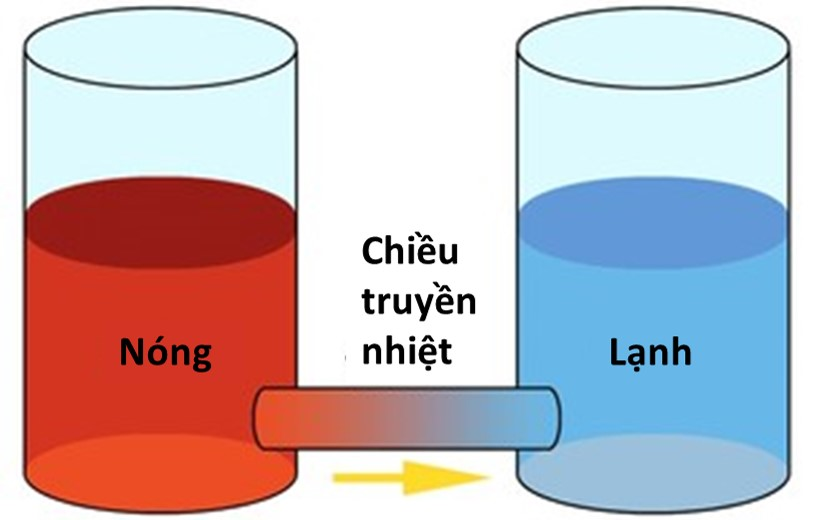
\includegraphics[width=0.3\linewidth]{figs/VN12-Y24-PH-SYL-002-1}
	\captionof{figure}{Minh hoạ chiều truyền nhiệt giữa hai vật có nhiệt độ khác nhau}
\end{center}
\subsubsection{Nhiệt độ}
\paragraph{Khái niệm về nhiệt độ}
\begin{boxdn}
	Nhiệt độ của một vật là đại lượng vật lí đặc trưng cho mức độ chuyển động nhiệt của phân tử vật chất cấu tạo nên vật. Khi các phân tử chuyển động nhiệt càng nhanh thì nhiệt độ của vật càng cao và ngược lại.
\end{boxdn}
\paragraph{Nhiệt kế}
\begin{boxdn}
	Nhiệt độ đo trên nhiệt kế được xác định thông qua giá trị của một đại lượng vật lí khác mà đại lượng này phụ thuộc theo nhiệt độ.
\end{boxdn}
\begin{boxvidu}
	\textbf{\textit{Ví dụ:}}
	\begin{itemize}
		\item Nhiệt kế thuỷ ngân xác định nhiệt độ dựa trên hiện tượng dãn nở vì nhiệt của thuỷ ngân.
		\item Nhiệt kế điện trở xác định nhiệt độ qua sự phụ thuộc của điện trở theo nhiệt độ.
	\end{itemize}
\end{boxvidu}
\begin{center}
	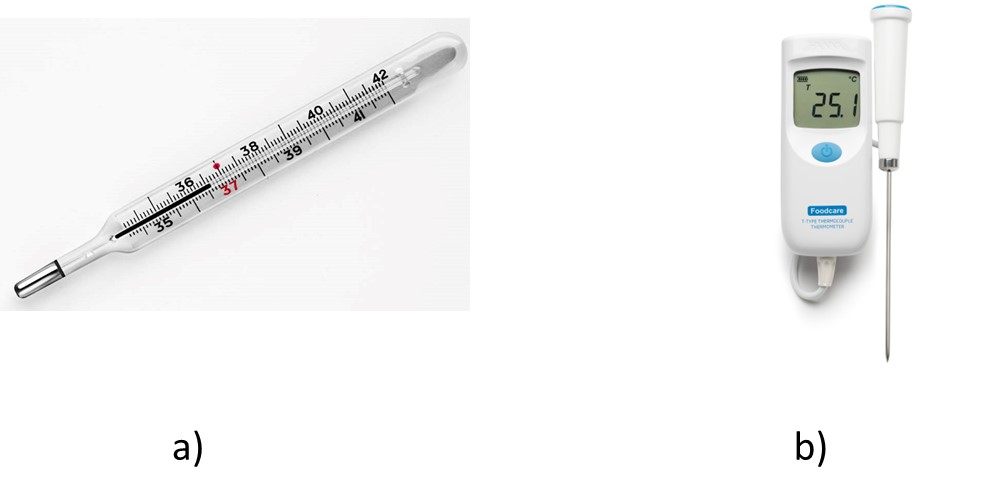
\includegraphics[width=0.5\linewidth]{figs/VN12-Y24-PH-SYL-002-2}
	\captionof{figure}{a) Nhiệt kế thuỷ ngân; b) Nhiệt kế điện trở}
\end{center}
\subsubsection{Thang nhiệt độ}
\paragraph{Thang nhiệt độ Celsius}
\begin{boxdn}
	Nhiệt độ trong thang đo này được kí hiệu là $t$. Đơn vị là độ Celsius (kí hiệu: $\si{\celsius}$).\\
	$\SI{1}{\celsius}=\dfrac{1}{100}$ của khoảng cách giữa nhiệt độ nóng chảy của nước tinh khiết đóng băng $\left(\SI{0}{\celsius}\right)$ và nhiệt độ sôi của nước tinh khiết ở áp suất $\SI{1}{atm}$ ($\SI{100}{\celsius}$).
\end{boxdn}

\paragraph{Thang nhiệt độ Kelvin}
\begin{boxdn}
	Nhiệt độ trong thang đo này được kí hiệu là $T$. Đơn vị là độ Kelvin (kí hiệu: $\si{\kelvin}$).\\
	$\SI{1}{\kelvin}=\dfrac{1}{273,15}$ của khoảng cách giữa nhiệt độ không tuyệt đối $\left(\SI{0}{\kelvin}\right)$ và nhiệt độ điểm mà nước tinh khiết tồn tại đồng thời ở thể rắn, lỏng và hơi ở áp suất $\SI{1}{atm}$ ($\SI{273.15}{\kelvin}$).\\
	Nhiệt độ không tuyệt đối ($\SI{0}{\kelvin}$) là nhiệt độ mà tại đó động năng chuyển động nhiệt của các phân tử cấu tạo nên vật chất bằng không và thế năng của chúng là tối thiểu.
\end{boxdn}
\begin{luuy}
	Một độ chia trên thang nhiệt độ Kelvin bằng một độ chia trên thang nhiệt độ Celsius.
\end{luuy}
\paragraph{Chuyển đổi nhiệt độ đo theo thang Celsius sang nhiệt độ đo theo thang Kelvin}
\begin{boxdl}
	\begin{equation}
		T=t+273,15\approx t+273
	\end{equation}
\end{boxdl}
với:
\begin{itemize}
	\item $t$: giá trị nhiệt độ của vật theo thang nhiệt độ Celsius;
	\item $T$: giá trị nhiệt độ của vật theo thang nhiệt độ Kelvin.
\end{itemize}
\subsection{VÍ DỤ MINH HOẠ}
\begin{dang}{Chuyển đổi được nhiệt độ đo theo thang Celsius sang nhiệt độ đo theo thang Kelvin và ngược lại}

\end{dang}
	\begin{vd}
Nhiệt độ của khối khí trong phòng đo được là $\SI{27}{\celsius}$. Xác định nhiệt độ của khối khí trong thang nhiệt độ Kelvin.
		\loigiai{
			Nhiệt độ khối khí trong thang nhiệt độ Kelvin:
			$$T=t+273=\SI{300}{\kelvin}.$$}
		
	
\end{vd}

\begin{vd}
	Một nhiệt kế dùng để đo nhiệt độ của các lò nung có phạm vi đo từ $\SI{263}{\kelvin}$ đến $\SI{1273}{\kelvin}$.
	\begin{enumerate}[label=\alph*)]
		\item Xác định phạm vi đo của nhiệt kế này trong thang nhiệt độ Celsius?
		\item Nếu sử dụng nhiệt kế này để đo nhiệt độ lò nung đang nấu chảy đồng có nhiệt độ nóng chảy là $\SI{1083}{\celsius}$ thì nhiệt kế có đo được không? Vì sao? Em có khuyến cáo gì về việc sử dụng nhiệt kế trong tình huống này?
	\end{enumerate}
	\loigiai{
		\begin{enumerate}[label=\alph*)]
			\item $t_\text{min}=T_\text{min}-273=\SI{-10}{\celsius};\quad t_\text{max}=T_\text{max}-273=\SI{1000}{\celsius}.$\\
			Phạm vi đo của nhiệt kế này trong thang nhiệt độ Celsius là $\SI{-10}{\celsius}$ đến $\SI{1000}{\celsius}$.
			\item Nếu sử dụng nhiệt kế này để đo nhiệt độ lò nung đang nấu chảy đồng có nhiệt độ nóng chảy $\SI{1083}{\celsius}$ thì nhiệt kế không đo được vì nhiệt độ cần đo nằm khoảng phạm vi đo của nhiệt kế.\\
			Trong trường hợp này, người đo cần dùng nhiệt kế có thang đo lớn hơn $\SI{1083}{\celsius}$ như nhiệt kế điện trở.
	\end{enumerate}}
\end{vd}

\begin{vd}
	Trong thang nhiệt độ Fahrenheit, chọn nhiệt độ tại điểm nước đá đang tan là $\SI{32}{\degree F}$, nhiệt độ tại điểm nước sôi ở điều kiện thường $\left(\SI{1}{atm}\right)$ là $\SI{212}{\degree F}$, trong khoảng nhiệt độ này chia thành 180 khoảng bằng nhau, mỗi khoảng ứng với $\SI{1}{\degree F}$. Thang đo này được nhà vật lí người Đức Daniel Gabriel Fahrenheit đề xuất vào năm 1724 và được sử dụng phổ biến ở các nước phương Tây. Nếu gọi $t$ là nhiệt độ của vật trong thang nhiệt độ Celsius và $T_\text{F}$ nhiệt độ của vật trong thang nhiệt độ Fahrenheit thì:
	$$T_\text{F}=a\cdot t+b.$$
	với $a$ và $b$ là các hệ số tỉ lệ.
	\begin{enumerate}[label=\alph*)]
		\item Em hãy xác định xác giá trị của $a$ và $b$.
		\item Trên tin tức thông báo nhiệt độ tại New York ngày 17/03/2024 là $\SI{49}{\degree F}$. Trong thang Celsius thì nhiệt độ này là bao nhiêu $\si{\celsius}$?
	\end{enumerate}
	\loigiai{
		\begin{enumerate}[label=\alph*)]
			\item Nhiệt độ tại điểm nước đá đang tan là $\SI{32}{\degree F}$ hay $\SI{0}{\celsius}$:
			\begin{equation}
				\label{eq: 1}\\
				b=\SI{32}{\degree F}
			\end{equation}
			Nhiệt độ tại điểm nước sôi ở điều kiện thường $\left(\SI{1}{atm}\right)$ là $\SI{212}{\degree F}$ hay $\SI{100}{\celsius}$:
			\begin{equation}
				\label{eq: 2}\\
				212=100a+b
			\end{equation}
			Từ (\ref{eq: 1}) và (\ref{eq: 2}), suy ra:
			\begin{equation*}
				\begin{cases}
					b=\SI{32}{\degree F}\\
					a=\SI{1.8}{\degree F/\celsius}
				\end{cases}
			\end{equation*}
			Như vậy, $T_\text{F}=1,8\cdot t+32.$
			\item Nhiệt độ tại New York ngày 17/03/2024 theo thang Celsius:
			$$t=\dfrac{T_\text{F}-32}{1,8}\approx\SI{9.44}{\celsius}.$$
	\end{enumerate}}
\end{vd}
\begin{luuy}
	$$\dfrac{t\left(\si{\degree F}\right)-32}{212-32}=\dfrac{t\left(\si{\celsius}\right)-0}{100-0}=\dfrac{T\left(\si{\kelvin}\right)-273}{373-273}.$$
\end{luuy}
\subsection{BÀI TẬP TRẮC NGHIỆM}
\inputansbox{10}{ans/G12Y24B2TN}
\Opensolutionfile{ans}[ans/G12Y24B2TN]
\begin{ex}
	Cho hai vật có nhiệt độ khác nhau tiếp xúc với nhau. Nhiệt được truyền từ
	\choice
	{vật có khối lượng lớn hơn sang vật có khối lượng nhỏ hơn}
	{\True vật có nhiệt độ cao hơn sang vật có nhiệt độ thấp hơn}
	{vật ở trên cao sang vật ở dưới thấp}
	{vật có khối lượng riêng lớn sang vật có khối lượng riêng nhỏ}
	\loigiai{

}
	\end{ex}
%====================================================================================
\begin{ex}
Người ta cho hai vật dẫn nhiệt A và B tiếp xúc với nhau, sau một thời gian khi có trạng thái cân bằng nhiệt thì hai vật này có
	\choice
	{\True cùng nhiệt độ}
	{cùng nội năng}
	{cùng năng lượng}
	{cùng nhiệt lượng}
	\loigiai{
	
}
\end{ex}

%====================================================================================
\begin{ex}
Đơn vị đo nhiệt độ trong thang nhiệt Celsius là
	\choice
	{$\si{\kelvin}$}
	{$\si{\degree F}$}
	{$\si{\newton}$}
	{\True $\si{\celsius}$}
	\loigiai{
		
	}
\end{ex}
%====================================================================================
\begin{ex}
	Nhiệt kế chất lỏng được chế tạo dựa trên nguyên tắc nào?
	\choice
	{\True Sự nở vì nhiệt của chất lỏng}
	{Sự phụ thuộc của tốc độ dòng chảy theo nhiệt độ}
	{Sự thay đổi điện trở của khối chất lỏng theo nhiệt độ}
	{Sự phụ thuộc của áp suất chất lỏng theo nhiệt độ}
	\loigiai{
		
	}
\end{ex}
%====================================================================================
\begin{ex}
Trong các nhiệt kế sau đây, em hãy chọn nhiệt kế phù hợp để đo nhiệt độ của nước đang được đun sôi?
	\choice
	{Nhiệt kế y tế có thang chia độ từ $\SI{35}{\celsius}$ đến $\SI{42}{\celsius}$}
	{ Nhiệt kế rượu có thang chia độ từ $\SI{-30}{\celsius}$ đến $\SI{60}{\celsius}$}
	{\True Nhiệt kế thuỷ ngân có thang chia độ từ $\SI{-10}{\celsius}$ đến $\SI{110}{\celsius}$}
	{Nhiệt kế hồng ngoại có thang chia độ từ $\SI{30}{\celsius}$ đến $\SI{45}{\celsius}$}
	\loigiai{
		
	}
\end{ex}
%====================================================================================
\begin{ex}
	Cách xác định nhiệt độ trong thang nhiệt độ Celsius là
	\choice
	{Lấy nhiệt độ của nước khi đóng băng là $\left(\SI{10}{\celsius}\right)$ và nhiệt độ sôi của nước $\left(\SI{100}{\celsius}\right)$ làm chuẩn}
	{Lấy nhiệt độ của nước khi đóng băng là $\left(\SI{100}{\celsius}\right)$ và nhiệt độ sôi của nước $\left(\SI{0}{\celsius}\right)$ làm chuẩn}
	{\True Lấy nhiệt độ của nước khi đóng băng là $\left(\SI{0}{\celsius}\right)$ và nhiệt độ sôi của nước $\left(\SI{100}{\celsius}\right)$ làm chuẩn}
	{Lấy nhiệt độ của nước khi đóng băng là $\left(\SI{100}{\celsius}\right)$ và nhiệt độ sôi của nước $\left(\SI{10}{\celsius}\right)$ làm chuẩn}
	\loigiai{
		
	}
\end{ex}
%====================================================================================
\begin{ex}
	Điểm đóng băng và sôi của nước theo thang Kelvin là
	\choice
	{$\SI{0}{\kelvin}$ và $\SI{100}{\kelvin}$}
	{\True $\SI{273}{\kelvin}$ và $\SI{373}{\kelvin}$}
	{$\SI{37}{\kelvin}$ và $\SI{73}{\kelvin}$}
	{$\SI{32}{\kelvin}$ và $\SI{212}{\kelvin}$}
	\loigiai{
		
	}
\end{ex}

%====================================================================================
\begin{ex}
	Độ không tuyệt đối là nhiệt độ ứng với
	\choice
	{\True $\SI{0}{\kelvin}$}
	{$\SI{0}{\celsius}$}
	{$\SI{273}{\kelvin}$}
	{$\SI{273}{\celsius}$}
	\loigiai{
		
	}
\end{ex}
%====================================================================================
\begin{ex}
	Chọn phát biểu \textbf{đúng}.\\
	Nhiệt độ không tuyệt đối là nhiệt độ mà tại đó
	\choice
	{\True chuyển động nhiệt của phân tử hầu như dừng lại}
	{nước bắt đầu đông thành đá}
	{tất cả chất khí hoá lỏng}
	{tất cả chất khí hoá rắn}
	\loigiai{
		
	}
\end{ex}
%====================================================================================
\begin{ex}
Không thể dùng nhiệt kế rượu để đo nhiệt độ của nước đang sôi vì
	\choice
	{rượu sôi ở nhiệt độ cao hơn $\SI{100}{\celsius}$}
	{\True rượu sôi ở nhiệt độ thấp hơn $\SI{100}{\celsius}$}
	{rượu đông đặc ở nhiệt độ $\SI{100}{\celsius}$}
	{rượu đông đặc ở nhiệt độ thấp hơn $\SI{0}{\celsius}$}
	\loigiai{
		
	}
\end{ex}
%====================================================================================
\begin{ex}
Biểu thức nào sau đây là đúng khi biến đổi nhiệt độ từ thang Celsius sang thang Kelvin?
	\choice
	{$T\left(\si{\kelvin}\right)=t\left(\si{\celsius}\right)-273$}
	{\True $T\left(\si{\kelvin}\right)=t\left(\si{\celsius}\right)+273$}
	{$T\left(\si{\kelvin}\right)=\dfrac{t\left(\si{\celsius}\right)+273}{2}$}
	{$T\left(\si{\kelvin}\right)=2t\left(\si{\celsius}\right)+273$}
	\loigiai{
		
	}
\end{ex}
%====================================================================================
\begin{ex}
Cho các bước như sau:
\begin{enumerate}[label=(\arabic*)]
	\item Thực hiện phép đo nhiệt độ.
	\item Ước lượng nhiệt độ của vật.
	\item Hiệu chỉnh nhiệt kế.
	\item Lựa chọn nhiệt kế phù hợp.
	\item Đọc và ghi kết quả đo.
\end{enumerate}
Các bước đúng khi thực hiện đo nhiệt độ của một vật là
	\choice
	{\True (2), (4), (3), (1), (5)}
	{(1), (4), (2), (3), (5)}
	{(1), (2), (3), (4), (5)}
	{(3), (2), (4), (1), (5)}
	\loigiai{
		
	}
\end{ex}
%====================================================================================
\begin{ex}
Nhiệt độ trung bình của nước ở thang nhiệt độ Celsius là $\SI{27}{\celsius}$ ứng với thang nhiệt độ Kelvin thì nhiệt độ của nước là
	\choice
	{$\SI{273}{\kelvin}$}
	{\True $\SI{300}{\kelvin}$}
	{$\SI{246}{\kelvin}$}
	{$\SI{327}{\kelvin}$}
	\loigiai{
			$$T=t+273=\SI{300}{\kelvin}.$$
	}
\end{ex}
%====================================================================================
\begin{ex}
Nhiệt độ mùa đông tại thành phố New York (Mỹ) là $\SI{283}{\kelvin}$, ứng với nhiệt giai Celsius thì nhiệt độ ở đó là
	\choice
	{\True $\SI{10}{\celsius}$}
	{$\SI{-10}{\celsius}$}
	{$\SI{5}{\celsius}$}
	{$\SI{-5}{\celsius}$}
	\loigiai{
		$$t=T-273=\SI{10}{\celsius}.$$
	}
\end{ex}


%====================================================================================
\begin{ex}
	Nhiệt độ vào một ngày mùa hè ở thành phố Hồ Chí Minh là $\SI{35}{\celsius}$. Nhiệt độ đó tương ứng với bao nhiêu độ $\si{\degree F}$?
	\choice
	{$\SI{59}{\degree F}$}
	{$\SI{67}{\degree F}$}
	{\True $\SI{95}{\degree F}$}
	{$\SI{76}{\degree F}$}
	\loigiai{
		$$t\left(\si{\degree F}\right)=32+1,8t\left(\si{\celsius}\right)=\SI{95}{\degree F}.$$
	}
\end{ex}
%====================================================================================
\begin{ex}
	Giá trị nhiệt độ đo được theo thang nhiệt độ Kelvin là $\SI{293}{\kelvin}$. Tính theo thang nhiệt độ Fahrenheit, nhiệt độ đó có giá trị là
	\choice
	{$\SI{20}{\degree F}$}
	{$\SI{100}{\degree F}$}
	{\True $\SI{68}{\degree F}$}
	{$\SI{261}{\degree F}$}
	\loigiai{
		$$t\left(\si{\celsius}\right)=T-273=\SI{20}{\celsius}.$$
	$$t\left(\si{\degree F}\right)=32+1,8t\left(\si{\celsius}\right)=\SI{68}{\degree F}.$$}
\end{ex}
%====================================================================================
\begin{ex}
	$\SI{104}{\degree F}$ ứng với bao nhiêu độ Kelvin?
	\choice
	{\True $\SI{313}{\kelvin}$}
	{$\SI{298}{\kelvin}$}
	{$\SI{328}{\kelvin}$}
	{$\SI{293}{\kelvin}$}
	\loigiai{
		$$\dfrac{t\left(\si{\degree F}\right)-32}{212-32}=\dfrac{T\left(\si{\kelvin}\right)-273}{373-273}$$
		Thay $t\left(\si{\degree F}\right)=\SI{104}{\degree F}$, thu được $T=\SI{313}{\kelvin}.$}
	\end{ex}
%====================================================================================
\begin{ex}
	Một thang đo $X$ lấy điểm đóng băng là $-10X$, lấy điểm sôi là $90X$. Nhiệt độ của một vật đọc được trên theo nhiệt giai Celsius là $\SI{40}{\celsius}$ thì trong nhiệt giai $X$ có nhiệt độ bằng
	\choice
	{$20X$}
	{\True $30X$}
	{$40X$}
	{$50X$}
	\loigiai{
		Độ chênh lệch nhiệt độ tại điểm băng và điểm sôi trong thang X cũng là 100. Như vậy $\SI{1}{\celsius}$ tương ứng với $\SI{1}{X}$ và
		$$t\left(\si{\celsius}\right)=t\left(\si{X}\right)+10.$$
	}
\end{ex}
%====================================================================================
\begin{ex}
	Giả sử có một thang nhiệt độ kí hiệu Z. Nhiệt độ sôi của nước theo thang này là $60Z$, điểm ba cả nước là $-15Z$. Nhiệt độ của vật theo thang Fahrenheit là bao nhiêu nếu nhiệt độ trong thang Z là $-96Z$?Giả sử có một thang nhiệt độ kí hiệu Z. Nhiệt độ sôi của nước theo thang này là $60Z$, điểm ba cả nước là $-15Z$. Nhiệt độ của vật theo thang Fahrenheit là bao nhiêu nếu nhiệt độ trong thang Z là $-96Z$?
	\choice
	{$\SI{-62.4}{\degree F}$}
	{$\SI{162.4}{\degree F}$}
	{\True $\SI{-162.4}{\degree F}$}
	{$\SI{62.4}{\degree F}$}
	\loigiai{
	$$\dfrac{t\left(\si{\degree F}\right)-32}{212-32}=\dfrac{Z-\left(-15\right)}{60-\left(-15\right)}$$
	Thay $Z=-96$ ta thu được $t\left(\si{\degree F}\right)=\SI{-162.4}{\degree F}.$
	}
\end{ex}
%====================================================================================
\begin{ex}
Hình dưới thể hiện nhiệt kế đo nhiệt độ của một vật. Sai số dụng cụ được lấy bằng một nửa độ chia nhỏ nhất. Kết quả đo nhiệt độ của vật này là
\begin{center}
	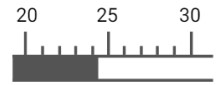
\includegraphics[width=0.25\linewidth]{figs/VN12-Y24-PH-SYL-002P-3}
\end{center}
	\choice
	{\True $t=\xsi{24.0\pm0.5}{\celsius}$}
	{$t=\xsi{25.0\pm0.5}{\celsius}$}
	{$t=\xsi{24.0\pm1.0}{\celsius}$}
	{$t=\xsi{25.0\pm1.0}{\celsius}$}
	\loigiai{
		
	}
\end{ex}

%====================================================================================
\begin{ex}
Chiều dài của phần thuỷ ngân trong nhiệt kế là $\SI{2}{\centi\meter}$ ở $\SI{0}{\celsius}$ và $\SI{22}{\centi\meter}$ ở $\SI{100}{\celsius}$. Nhiệt độ là bao nhiêu nếu chiều dài của thuỷ ngân là $\SI{8}{\centi\meter}$?
	\choice
	{$\SI{40}{\celsius}$.$\SI{40}{\celsius}$}
	{$\SI{50}{\celsius}$}
	{$\SI{20}{\celsius}$}
	{\True $\SI{30}{\celsius}$}
	\loigiai{
		$$\dfrac{\ell-\ell_0}{t-t_0}=\dfrac{\ell'-\ell_0}{t'-t_0}$$
		$$\Leftrightarrow\dfrac{\SI{22}{\centi\meter}-\SI{2}{\centi\meter}}{\SI{100}{\celsius}-\SI{0}{\celsius}}=\dfrac{\SI{8}{\centi\meter}-\SI{2}{\centi\meter}}{t'-\SI{0}{\celsius}}\Rightarrow t'=\SI{30}{\celsius}.$$
	}
\end{ex}
%====================================================================================
\begin{ex}
Chiều dài của phần thuỷ ngân trong nhiệt kế là $\SI{2}{\centi\meter}$ ở $\SI{0}{\celsius}$ và $\SI{22}{\centi\meter}$ ở $\SI{100}{\celsius}$. Chiều dài của phần thuỷ ngân sẽ là bao nhiêu nếu nhiệt độ là $\SI{50}{\celsius}$?
	\choice
	{$\SI{10}{\centi\meter}$}
	{\True $\SI{12}{\centi\meter}$}
	{$\SI{14}{\centi\meter}$}
	{$\SI{16}{\centi\meter}$}
	\loigiai{
	$$\dfrac{\ell-\ell_0}{t-t_0}=\dfrac{\ell'-\ell_0}{t'-t_0}$$
	$$\Leftrightarrow\dfrac{\SI{22}{\centi\meter}-\SI{2}{\centi\meter}}{\SI{100}{\celsius}-\SI{0}{\celsius}}=\dfrac{\ell'-\SI{2}{\centi\meter}}{\SI{50}{\celsius}-\SI{0}{\celsius}}\Rightarrow \ell'=\SI{12}{\centi\meter}.$$
	}
\end{ex}
%====================================================================================
\begin{ex}
Sự phụ thuộc vào nhiệt độ của bước sóng điện từ theo hệ thức Wien: $T\cdot\lambda_\text{max}=\SI{2900}{\left(\micro\meter\cdot\kelvin\right)}$ được dùng vào việc chế tạo các nhiệt kế thường dùng hằng ngày như
nhiệt kế hồng ngoại, cũng như các nhiệt kế trong thiên văn để đo nhiệt độ bề mặt của
các thiên thể. Xét một nhiệt kế hồng ngoại khi đo nhiệt độ cơ thể người như hình vẽ.
Bước sóng hồng ngoại do cơ thể người phát ra bằng xấp xỉ bằng
\begin{center}
	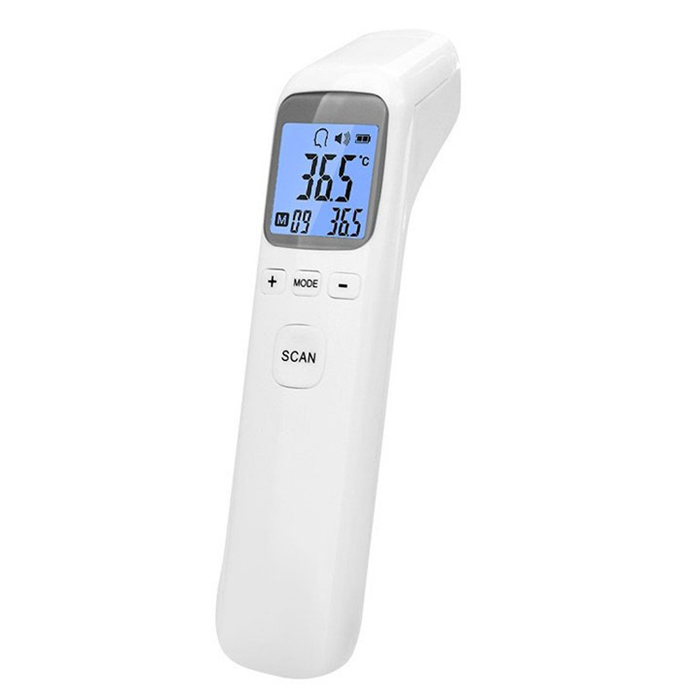
\includegraphics[width=0.3\linewidth]{figs/VN12-Y24-PH-SYL-002P-1}
\end{center}
	\choice
	{\True $\SI{9.4}{\micro\meter}$}
	{$\SI{79}{\micro\meter}$}
	{$\SI{29}{\micro\meter}$}
	{$\SI{10.6}{\micro\meter}$}
	\loigiai{
	$$\lambda_\text{max}=\dfrac{\SI{2900}{\micro\meter\cdot\kelvin}}{T}=\dfrac{\SI{2900}{\micro\meter\cdot\kelvin}}{36,5+\SI{273}{\kelvin}}\approx\SI{9.4}{\micro\meter}.$$
	}
\end{ex}
\Closesolutionfile{ans}
\subsection{TRẮC NGHIỆM ĐÚNG/SAI}
\setcounter{ex}{0}

\begin{ex}
		Bảng sau đây ghi sự thay đổi nhiệt độ của không khí theo thời gian dựa trên số liệu của một trạm khí tượng ở Hà Nội ghi được vào một ngày mùa đông.
	\begin{center}
		\begin{tabular}{|C{8em}|C{1.5em}|C{1.5em}|C{1.5em}|C{1.5em}|C{1.5em}|C{1.5em}|C{1.5em}|C{1.5em}|}
			\hline
			\thead{Thời gian (giờ)}& 1 & 4 & 7 & 10 & 13 & 16 & 19 & 22\\
			\hline
			\thead{Nhiệt độ $\left(\si{\celsius}\right)$} & 13 & 13 &13 & 18& 18 & 20 & 17 & 12\\
			\hline
		\end{tabular}
	\end{center}
	\begin{enumerate}[label=\alph*)]
		\item Nhiệt độ lúc 4 giờ là $\SI{286}{\kelvin}$.
		\item Nhiệt độ thấp nhất trong ngày là vào lúc 1 giờ.
		\item Nhiệt độ cao nhất trong ngày là vào lúc 16 giờ.
		\item Độ chênh lệch nhiệt độ trong ngày là $\SI{6}{\celsius}$.
	\end{enumerate}
	\loigiai{
	\begin{enumerate}[label=\alph*)]
		\item Đúng.
		\item Sai. Nhiệt độ thấp nhất là $\SI{12}{\celsius}$ vào lúc $\SI{22}{\hour}$.
		\item Đúng.
		\item Sai. Độ chênh lệch nhiệt độ trong ngày là $\SI{8}{\celsius}$.
	\end{enumerate}
	
}
	\end{ex}

% =================================================================================
\begin{ex}
	Bảng dưới đây ghi tên các loại nhiệt kế và thang đo của chúng
	\begin{center}
		\begin{tabular}{|C{5cm}|C{6cm}|}
			\hline
			\thead{Loại nhiệt kế} & \thead{Thang nhiệt độ}\\
			\hline
			Thuỷ ngân & Từ $\SI{-10}{\celsius}$ đến $\SI{110}{\celsius}$\\
			\hline
			Rượu & Từ $\SI{-30}{\celsius}$ đến $\SI{60}{\celsius}$\\
			\hline
			Kim loại & Từ $\SI{0}{\celsius}$ đến $\SI{400}{\celsius}$\\
			\hline
			Điện tử & Từ $\SI{34}{\celsius}$ đến $\SI{42}{\celsius}$\\
			\hline
		\end{tabular}
	\end{center}
	\begin{enumerate}[label=\alph*)]
		\item Dùng nhiệt kế kim loại để đo nhiệt độ nước sôi.
		\item Dùng nhiệt kế điện tử để đo nhiệt độ cơ thể người.
		\item Dùng nhiệt kế thuỷ ngân để đo nhiệt độ không khí trong phòng.
		\item Dùng nhiệt kế rượu để đo nhiệt độ bề mặt bàn là.
	\end{enumerate}
	\loigiai{
	\begin{enumerate}[label=\alph*)]
		\item Đúng.
		\item Đúng.
		\item Đúng.
		\item Sai.
	\end{enumerate}
}
	\end{ex}
% ================================================================================
	\begin{ex}
		Hình bên là một nhiệt kế rượu.
		\begin{center}
			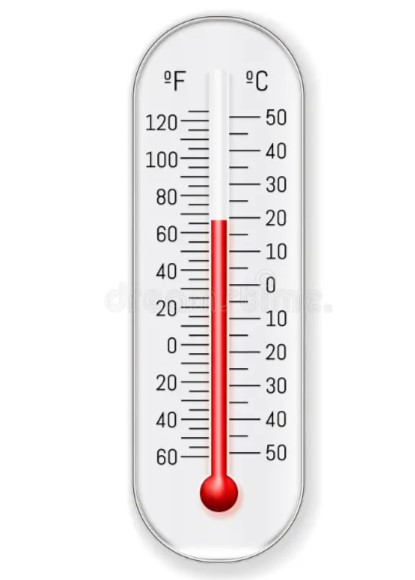
\includegraphics[width=0.25\linewidth]{figs/VN12-Y24-PH-SYL-002P-2}
		\end{center}
		\begin{enumerate}[label=\alph*)]
			\item Giới hạn đo của nhiệt kế là $\SI{120}{\celsius}$.
			\item Độ chia nhỏ nhất của nhiệt kế là $\SI{5}{\celsius}$.
			\item Nhiệt độ hiện tại trên nhiệt kế là $\SI{19}{\celsius}$.
			\item Có thể dùng nhiệt kế để xác định nhiệt độ của nước sôi.
		\end{enumerate}
		\loigiai{
		\begin{enumerate}[label=\alph*)]
			\item Sai. Giới hạn đo của nhiệt kế là $\SI{50}{\celsius}$.
			\item Đúng.
			\item Sai. ĐCNN của nhiệt kế là $\SI{5}{\celsius}$ nên không thể đọc được giá trị $\SI{19}{\celsius}$, nhiệt độ hiện tại có thể đọc từ nhiệt kế là $\SI{20}{\celsius}$.
			\item Sai. Giới hạn đo của nhiệt kế nhỏ hơn nhiệt độ nước sôi.
		\end{enumerate}
	}

		\end{ex}
\subsection{BÀI TẬP TỰ LUẬN}
\setcounter{ex}{0}
\begin{ex}
	Theo dự báo thời tiết ngày 17/04/2024 thì nhiệt độ trung bình ngày - đêm trong
	ngày hôm đó tại Thành phố Hồ Chí Minh là  $\SI{35}{\celsius}-\SI{25}{\celsius}$. Sự chênh lệch nhiệt độ này trong thang đo Kelvin là bao nhiêu $\si{\kelvin}$?
	\loigiai{
		$$\Delta T=\SI{10}{\kelvin}.$$	
}
	\end{ex}

% ===================================================================================
\begin{ex}
	Thế giới từng ghi nhận sự thay đổi nhiệt độ rất lớn diễn ra ở Spearfish, South Dakota vào ngày 22/01/1943. Lúc 7h30 sáng, nhiệt độ ngoài trời là $\SI{-20}{\celsius}$. Hai phút sau, nhiệt độ ngoài trời tăng lên đến $\SI{7.2}{\celsius}$. Xác định độ tăng nhiệt độ trung bình trong 2 phút đó theo đơn vị Kelvin/giây.
	\loigiai{
		$$\dfrac{\Delta T}{t}=\dfrac{\SI{27.2}{\kelvin}}{\SI{120}{\second}}\approx\SI{0.23}{\kelvin/\second}.$$
	}
	\end{ex}
% ===================================================================================
\begin{ex}
Ở $\SI{20}{\celsius}$ một thanh nhôm dài $\SI{12}{\meter}$. Tính nhiệt độ cần thiết để chiều dài thanh nhôm là $\SI{12.01}{\meter}$. Biết rằng khi nhiệt độ tăng thêm $\SI{1}{\celsius}$ thì thanh nhôm dài thêm $\SI{2.3E-5}{}$ chiều dài ban đầu.
\loigiai{
	$$\Delta\ell=\alpha\ell_0\Delta t$$
	với $\alpha=\SI{2.3E-5}{\kelvin^{-1}}$.
	$$\Rightarrow \Delta t=\dfrac{\Delta \ell}{\alpha\ell_0}=\SI{36.23}{\celsius}.$$
	Vậy nhiệt độ cần thiết để thanh nhôm dài $\SI{12.01}{\meter}$ là $\SI{56.23}{\celsius}$.
}
\end{ex}


% ===================================================================================
\begin{ex}
Một nhiệt kế thể tích không đổi hiển thị nhiệt độ $\SI{0}{\celsius}$ và $\SI{100}{\celsius}$ với các áp suất $\SI{60}{\centi\meter Hg}$ và $\SI{120}{\centi\meter Hg}$. Biết nhiệt độ đọc được là hàm bậc nhất của áp suất. Khi áp suất thuỷ ngân là $\SI{90}{\centi\meter Hg}$ thì nhiệt độ đọc được bằng bao nhiêu?
\loigiai{
	Ta có:
	$$t=a\cdot p+b\Rightarrow \dfrac{t-t_1}{t_2-t_1}=\dfrac{p-p_1}{p_2-p_1}.$$
	Thay $p=\SI{90}{\centi\meter Hg}$; $t_1=\SI{0}{\celsius}$; $t_2=\SI{100}{\celsius}$; $p_1=\SI{60}{\centi\meter Hg}$; $p_2=\SI{120}{\centi\meter Hg}$, ta thu được: $t=\SI{50}{\celsius}.$
}

\end{ex}



